% BEGIN TEMPLATE
\documentclass[11pt]{article}
\usepackage{graphicx}
\usepackage{hyperref} 
\usepackage{xcolor}
\usepackage{nameref}
\usepackage{listings}
\usepackage{float}
\usepackage[title]{appendix}
\usepackage[ruled]{algorithm2e}
\graphicspath{ {../../images/} }
\bibliographystyle{acm}
% CHANGE THESE
\newcommand{\courseListing}{CSCI 8360}
\newcommand{\courseName}{Machine Learning for Text}
\newcommand{\assignmentTitle}{Summary \#3}
\newcommand{\assignmentSubtitle}{Python K-Means}
\usepackage{geometry}
\geometry{margin=1in}

\hypersetup{
    colorlinks,
    linkcolor={red!50!black},
    citecolor={blue!50!black},
    urlcolor={blue!80!black}
}
\urlstyle{same}
\definecolor{codegreen}{rgb}{0,0.6,0}
\definecolor{codegray}{rgb}{0.5,0.5,0.5}
\definecolor{codepurple}{rgb}{0.58,0,0.82}
\lstdefinestyle{mystyle}{
    commentstyle=\color{codegreen},
    keywordstyle=\color{magenta},
    numberstyle=\tiny\color{codegray},
    stringstyle=\color{codepurple},
    basicstyle=\ttfamily\footnotesize,
    breakatwhitespace=false,         
    breaklines=true,                 
    captionpos=b,                    
    keepspaces=true,                 
    numbers=left,                    
    numbersep=5pt,                  
    showspaces=false,                
    showstringspaces=false,
    showtabs=false,                  
    tabsize=2
}

\lstset{style=mystyle}

\begin{document}
  \begin{center}
  
\includegraphics[scale=0.15]{UNO-Logo-Color.png}
  \\[0.3in]
  \textbf{\courseListing{}}\\
  \courseName{}
  \\[0.75in]
  \textbf{\assignmentTitle{}}\\
  \assignmentSubtitle{}
  \\[0.75in]
  \textbf{Patrick Davlin}
  \\[0.75in]
  \textbf{Computer Science Department}\\
  \textbf{Peter Kiewit Institute}\\
  \textbf{University of Nebraska}
  \\[0.75in]
  \textbf{Fall 2021}
  \\[0.3in]
  
\includegraphics[scale=0.075]{UNO-Icon-Color.png}
  \newpage
\end{center}
  \graphicspath{{./images/}}
\newpage
For this assignment, the primary task was to implement and observe the K-Means algorithm in Python.
In doing so, students were permitted to use any libraries necessary to implement the algorithm, with the intent being to observe the impact of various parameters on the algorithm.
With this in mind, a logical first step was to import the scikit-learn (\lstinline{sklearn}) package into the script and import its \lstinline{KMeans} subpackage.
This feels a bit like skipping to the end, but in the scope of the assignment was a sensible approach--the K-Means implementation in \lstinline{sklearn} is quite long--keeping in mind that the intent was to observe the algorithm in practice.
Handily, \lstinline{sklearn} also has the 20 newsgroup dataset built in as well.

Like any machine learning implementation, the first and most intensive part of this assignment was developing an understanding of what the data is and how to organize it for use with the applied model.
Approaching this, the first goal was to vectorize the incoming text for use in the K-Means model.
Fortunately, \lstinline{sklearn} contains a \lstinline{TfidfVectorizer} used to convert input text to a document-term matrix.
This is a difficult concept to understand, intuitively--the dimensionality of this matrix, according to the output of \lstinline{.shape()}, is \lstinline{(11314, 114441)}.
Interpreting this, there are 11,314 documents in the corpus, containing a total of 114,441 terms.
Immediately, this shape stands out--there are no doubt many extra terms used in this corpus that would be considered nonessential.
Therefore, the next step was to add a quick loop operation to reduce the number of stop words in the application, using a list of \lstinline{ENGLISH_STOP_WORDS} from the \lstinline{sklearn} package.
This can be found on lines 21-29 in the code found in the \nameref{codelist}.

Having vectorized data, it was then possible to use the K-Means algorithm to generate clusters of data.
From that, centroid locations can be observed, and resulting cluster labels can be used for visualization and discussion.
The final step toward visualizing the results was reducing the number of dimensions in the dataset to fit into a two-dimensional plot.
This was the most difficult part of the assignment, in terms of managing data and in learning to implement these methods.
Intuitively, one would expect that the output of the K-Means algorithm would be mappable on its own to the existing data, but this is not the case.
Looking through available \lstinline{sklearn} methods, a few stood out immediately.
The first of these was the Principal component analysis (\lstinline{PCA}) package, which has been used for assignments in other courses.
Using this package on its own throws an error about sparse matrixes.
When attempting to modify the data to fit in the \lstinline{PCA} method, the memory usage was so significant that it almost immediately crashed the runtime of any machine running the code; this was verified locally and online using Google Colab.
The \lstinline{PCA} error recommends using \lstinline{TruncatedSVD} or \lstinline{NMF} packages instead.
With this in mind, and without a particular preference for methods of reducing dimensionality, both were used and compared.

The K-Means algorithm was run on the newsgroup data for 5, 10, 20, and 30 clusters of data, and then plotted after dimension reduction using both aforementioned methods.
In general, there is a lot of overlap between these clusters.
This was concerning at first, and prompted a harder look at the data.
Ultimately, considering the significant topical overlap of the newsgroup categories, it was determined that the overlap was probably expected between clusters, since many individual text items might use similar terms, even across the varying categories.
The overlap generally increases in correlation to the number of clusters--there appeared to be more overlap for 30 clusters than 5.
This also aligns with intuition on clustering in a dataset with substantial similarity across terms.
Complete outputs of the models can be found in \nameref{outputs}.

Reflecting on this assignment, it is easy to see how an understanding of clustering further enhances my general understanding of machine learning and text analysis.
Particularly with an eye toward the major projects in this course, this understanding appears to be a good foundation upon which to build more sophisticated techniques and implementations.

\newpage
\begin{appendices}
\section{K-Means Visualizations} \label{outputs}

\begin{figure}[H]
\centering
\begin{subfigure}{\textwidth}
  \centering
  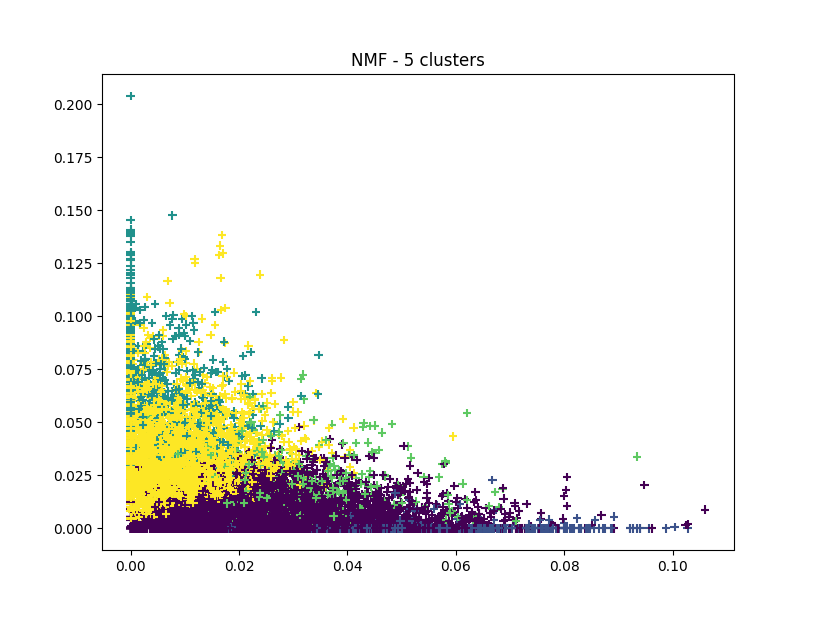
\includegraphics[width=3in]{images/nmf_5.png}
  \label{fig:nmf5}
\end{subfigure}%
\begin{subfigure}{\textwidth}
  \centering
  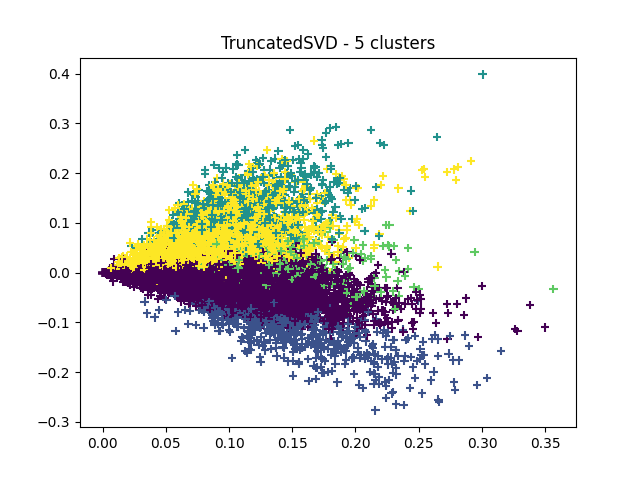
\includegraphics[width=3in]{images/svd_5.png}
  \label{fig:svd5}
\end{subfigure}
\caption{K = 5}
\label{fig:k5}
\end{figure}

\begin{figure}[H]
\centering
\begin{subfigure}{\textwidth}
  \centering
  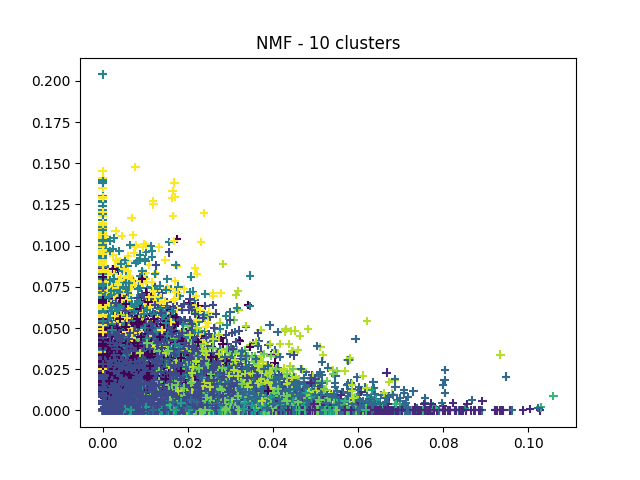
\includegraphics[width=3in]{images/nmf_10.png}
  \label{fig:nmf10}
\end{subfigure}%
\begin{subfigure}{\textwidth}
  \centering
  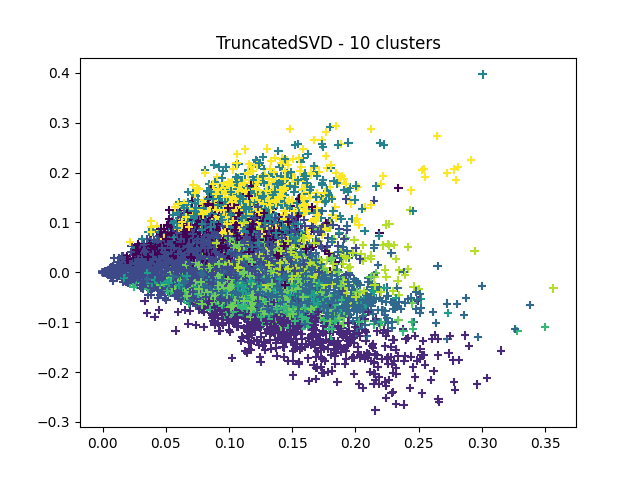
\includegraphics[width=3in]{images/svd_10.png}
  \label{fig:svd10}
\end{subfigure}
\caption{K = 10}
\label{fig:k10}
\end{figure}

\begin{figure}[H]
\centering
\begin{subfigure}{\textwidth}
  \centering
  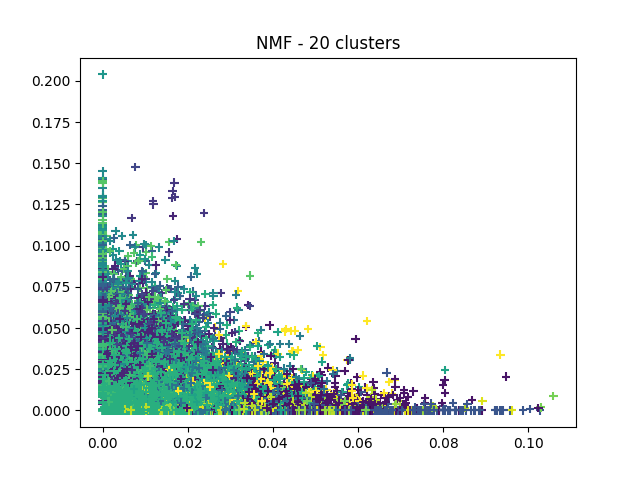
\includegraphics[width=3in]{images/nmf_20.png}
  \label{fig:nmf20}
\end{subfigure}%
\begin{subfigure}{\textwidth}
  \centering
  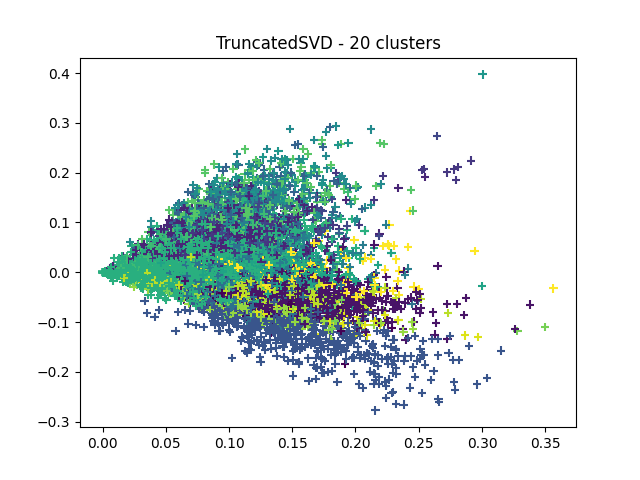
\includegraphics[width=3in]{images/svd_20.png}
  \label{fig:svd20}
\end{subfigure}
\caption{K = 20}
\label{fig:k20}
\end{figure}

\begin{figure}[H]
\centering
\begin{subfigure}{\textwidth}
  \centering
  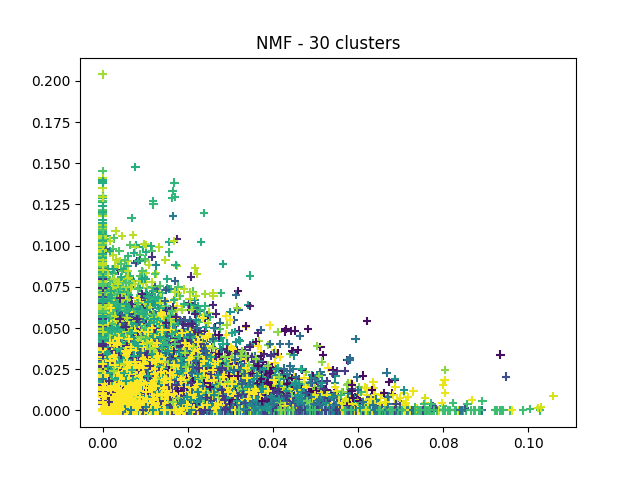
\includegraphics[width=3in]{images/nmf_30.png}
  \label{fig:nmf13}
\end{subfigure}%
\begin{subfigure}{\textwidth}
  \centering
  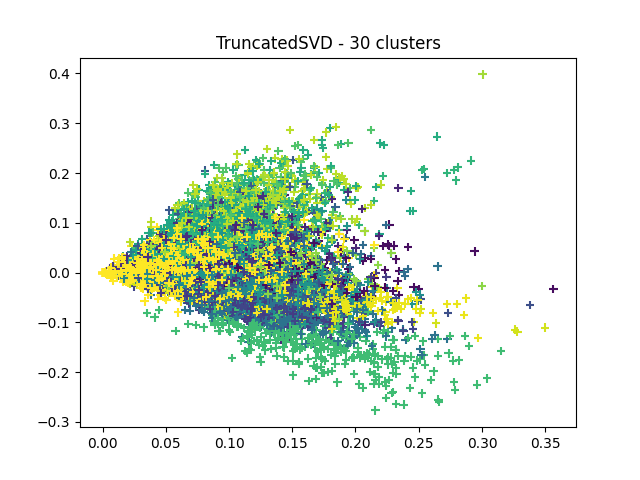
\includegraphics[width=3in]{images/svd_30.png}
  \label{fig:svd30}
\end{subfigure}
\caption{K = 30}
\label{fig:k30}
\end{figure}


\newpage
\section{Complete Code Listing} \label{codelist}
\lstinputlisting[language=Python]{k-means.py}

\end{appendices}
  
\end{document}